

\tikzset{every picture/.style={line width=0.75pt}} %set default line width to 0.75pt        

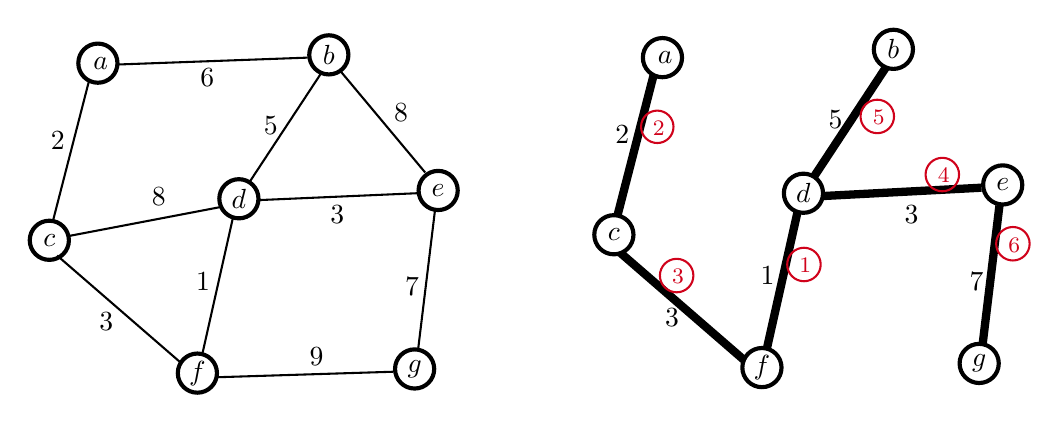
\begin{tikzpicture}[x=0.5pt,y=0.5pt,yscale=-1,xscale=1]
%uncomment if require: \path (0,294); %set diagram left start at 0, and has height of 294

%Straight Lines [id:da6859712806144006] 
\draw [color={rgb, 255:red, 0; green, 0; blue, 0 }  ,draw opacity=1 ][line width=0.75]    (237,42) -- (298,115) ;
%Straight Lines [id:da43828905709564314] 
\draw [color={rgb, 255:red, 0; green, 0; blue, 0 }  ,draw opacity=1 ][line width=0.75]    (147,263) -- (275,259) ;
%Straight Lines [id:da6385368954330931] 
\draw [color={rgb, 255:red, 0; green, 0; blue, 0 }  ,draw opacity=1 ][line width=0.75]    (32,175) -- (122,253) ;
%Straight Lines [id:da061278223687582845] 
\draw [color={rgb, 255:red, 0; green, 0; blue, 0 }  ,draw opacity=1 ][line width=0.75]    (40,161) -- (150,140) ;
%Straight Lines [id:da125058897644165] 
\draw [color={rgb, 255:red, 0; green, 0; blue, 0 }  ,draw opacity=1 ][line width=0.75]    (55,49) -- (29,150) ;
%Straight Lines [id:da7561477389708726] 
\draw [color={rgb, 255:red, 0; green, 0; blue, 0 }  ,draw opacity=1 ][line width=0.75]    (75,37) -- (213,32) ;
%Straight Lines [id:da8045438090716241] 
\draw [color={rgb, 255:red, 0; green, 0; blue, 0 }  ,draw opacity=1 ][line width=0.75]    (223,43) -- (171,122) ;
%Straight Lines [id:da7384444755679203] 
\draw [color={rgb, 255:red, 0; green, 0; blue, 0 }  ,draw opacity=1 ][line width=0.75]    (159,148) -- (137,246) ;
%Straight Lines [id:da7781378597799559] 
\draw [color={rgb, 255:red, 0; green, 0; blue, 0 }  ,draw opacity=1 ][line width=0.75]    (305,143) -- (293,242) ;
%Straight Lines [id:da6283012441188964] 
\draw [color={rgb, 255:red, 0; green, 0; blue, 0 }  ,draw opacity=1 ][line width=0.75]    (292,130) -- (177,135) ;
%Straight Lines [id:da8730022909148112] 
\draw [color={rgb, 255:red, 0; green, 0; blue, 0 }  ,draw opacity=1 ][line width=3]    (586,132) -- (700,126) ;
%Straight Lines [id:da5161692873874864] 
\draw [color={rgb, 255:red, 0; green, 0; blue, 0 }  ,draw opacity=1 ][line width=3]    (463,45) -- (437,146) ;
%Straight Lines [id:da4352724287531199] 
\draw [color={rgb, 255:red, 0; green, 0; blue, 0 }  ,draw opacity=1 ][line width=3]    (631,39) -- (579,118) ;
%Straight Lines [id:da4878171039675874] 
\draw [color={rgb, 255:red, 0; green, 0; blue, 0 }  ,draw opacity=1 ][line width=3]    (567,144) -- (545,242) ;
%Straight Lines [id:da9647292972064201] 
\draw [color={rgb, 255:red, 0; green, 0; blue, 0 }  ,draw opacity=1 ][line width=3]    (713,139) -- (701,238) ;
%Straight Lines [id:da358430115249718] 
\draw [color={rgb, 255:red, 0; green, 0; blue, 0 }  ,draw opacity=1 ][line width=3]    (439,173) -- (529,251) ;

% Text Node
\draw  [line width=1.5]   (307.38, 128) circle [x radius= 14.15, y radius= 14.15]   ;
\draw (307.38,128) node   [align=left] {$\displaystyle e$};
% Text Node
\draw  [line width=1.5]   (61.48, 36) circle [x radius= 14.15, y radius= 14.15]   ;
\draw (55.98,36) node [anchor=west] [inner sep=0.75pt]   [align=left] {$\displaystyle a$};
% Text Node
\draw  [line width=1.5]   (228.38, 30) circle [x radius= 14.15, y radius= 14.15]   ;
\draw (228.38,30) node   [align=left] {$\displaystyle b$};
% Text Node
\draw  [line width=1.5]   (26.38, 164) circle [x radius= 14.15, y radius= 14.15]   ;
\draw (26.38,164) node   [align=left] {$\displaystyle c$};
% Text Node
\draw  [line width=1.5]   (163.38, 134) circle [x radius= 14.15, y radius= 14.15]   ;
\draw (163.38,134) node   [align=left] {$\displaystyle d$};
% Text Node
\draw  [line width=1.5]   (133.38, 260) circle [x radius= 14.15, y radius= 14.15]   ;
\draw (133.38,260) node   [align=left] {$\displaystyle f$};
% Text Node
\draw  [line width=1.5]   (290.38, 257) circle [x radius= 14.15, y radius= 14.15]   ;
\draw (290.38,257) node   [align=left] {$\displaystyle g$};
% Text Node
\draw (25.24,83.06) node [anchor=north west][inner sep=0.75pt]   [align=left] {$\displaystyle 2$};
% Text Node
\draw (133.24,38.06) node [anchor=north west][inner sep=0.75pt]   [align=left] {$\displaystyle 6$};
% Text Node
\draw (227.24,137.06) node [anchor=north west][inner sep=0.75pt]   [align=left] {$\displaystyle 3$};
% Text Node
\draw (179.24,72.06) node [anchor=north west][inner sep=0.75pt]   [align=left] {$\displaystyle 5$};
% Text Node
\draw (98.24,124.06) node [anchor=north west][inner sep=0.75pt]   [align=left] {$\displaystyle 8$};
% Text Node
\draw (60.24,214.06) node [anchor=north west][inner sep=0.75pt]   [align=left] {$\displaystyle 3$};
% Text Node
\draw (130.24,185.06) node [anchor=north west][inner sep=0.75pt]   [align=left] {$\displaystyle 1$};
% Text Node
\draw (273.24,63.06) node [anchor=north west][inner sep=0.75pt]   [align=left] {$\displaystyle 8$};
% Text Node
\draw (212.24,239.06) node [anchor=north west][inner sep=0.75pt]   [align=left] {$\displaystyle 9$};
% Text Node
\draw (281.24,189) node [anchor=north west][inner sep=0.75pt]   [align=left] {$\displaystyle 7$};
% Text Node
\draw  [line width=1.5]   (715.38, 124) circle [x radius= 14.15, y radius= 14.15]   ;
\draw (715.38,124) node   [align=left] {$\displaystyle e$};
% Text Node
\draw  [line width=1.5]   (469.48, 32) circle [x radius= 14.15, y radius= 14.15]   ;
\draw (463.98,32) node [anchor=west] [inner sep=0.75pt]   [align=left] {$\displaystyle a$};
% Text Node
\draw  [line width=1.5]   (636.38, 26) circle [x radius= 14.15, y radius= 14.15]   ;
\draw (636.38,26) node   [align=left] {$\displaystyle b$};
% Text Node
\draw  [line width=1.5]   (434.38, 160) circle [x radius= 14.15, y radius= 14.15]   ;
\draw (434.38,160) node   [align=left] {$\displaystyle c$};
% Text Node
\draw  [line width=1.5]   (571.38, 130) circle [x radius= 14.15, y radius= 14.15]   ;
\draw (571.38,130) node   [align=left] {$\displaystyle d$};
% Text Node
\draw  [line width=1.5]   (541.38, 256) circle [x radius= 14.15, y radius= 14.15]   ;
\draw (541.38,256) node   [align=left] {$\displaystyle f$};
% Text Node
\draw  [line width=1.5]   (698.38, 253) circle [x radius= 14.15, y radius= 14.15]   ;
\draw (698.38,253) node   [align=left] {$\displaystyle g$};
% Text Node
\draw (433.24,79.06) node [anchor=north west][inner sep=0.75pt]   [align=left] {$\displaystyle 2$};
% Text Node
\draw (642.24,137.06) node [anchor=north west][inner sep=0.75pt]   [align=left] {$\displaystyle 3$};
% Text Node
\draw (587.24,68.06) node [anchor=north west][inner sep=0.75pt]   [align=left] {$\displaystyle 5$};
% Text Node
\draw (538.24,181.06) node [anchor=north west][inner sep=0.75pt]   [align=left] {$\displaystyle 1$};
% Text Node
\draw (689.24,185) node [anchor=north west][inner sep=0.75pt]   [align=left] {$\displaystyle 7$};
% Text Node
\draw  [color={rgb, 255:red, 208; green, 2; blue, 27 }  ,draw opacity=1 ]  (571.74, 181.5) circle [x radius= 12.1, y radius= 12.1]   ;
\draw (566.24,175) node [anchor=north west][inner sep=0.75pt]  [font=\footnotesize,color={rgb, 255:red, 208; green, 2; blue, 27 }  ,opacity=1 ] [align=left] {$\displaystyle 1$};
% Text Node
\draw  [color={rgb, 255:red, 208; green, 2; blue, 27 }  ,draw opacity=1 ]  (465.74, 82) circle [x radius= 11.72, y radius= 11.72]   ;
\draw (460.24,76) node [anchor=north west][inner sep=0.75pt]  [font=\footnotesize,color={rgb, 255:red, 208; green, 2; blue, 27 }  ,opacity=1 ] [align=left] {2};
% Text Node
\draw  [color={rgb, 255:red, 208; green, 2; blue, 27 }  ,draw opacity=1 ]  (624.74, 74.5) circle [x radius= 12.1, y radius= 12.1]   ;
\draw (619.24,68) node [anchor=north west][inner sep=0.75pt]  [font=\footnotesize,color={rgb, 255:red, 208; green, 2; blue, 27 }  ,opacity=1 ] [align=left] {$\displaystyle 5$};
% Text Node
\draw (469.24,211.06) node [anchor=north west][inner sep=0.75pt]   [align=left] {$\displaystyle 3$};
% Text Node
\draw  [color={rgb, 255:red, 208; green, 2; blue, 27 }  ,draw opacity=1 ]  (479.74, 189.5) circle [x radius= 12.1, y radius= 12.1]   ;
\draw (474.24,183) node [anchor=north west][inner sep=0.75pt]  [font=\footnotesize,color={rgb, 255:red, 208; green, 2; blue, 27 }  ,opacity=1 ] [align=left] {$\displaystyle 3$};
% Text Node
\draw  [color={rgb, 255:red, 208; green, 2; blue, 27 }  ,draw opacity=1 ]  (671.74, 116.5) circle [x radius= 12.1, y radius= 12.1]   ;
\draw (666.24,110) node [anchor=north west][inner sep=0.75pt]  [font=\footnotesize,color={rgb, 255:red, 208; green, 2; blue, 27 }  ,opacity=1 ] [align=left] {$\displaystyle 4$};
% Text Node
\draw  [color={rgb, 255:red, 208; green, 2; blue, 27 }  ,draw opacity=1 ]  (722.74, 166.5) circle [x radius= 12.1, y radius= 12.1]   ;
\draw (717.24,160) node [anchor=north west][inner sep=0.75pt]  [font=\footnotesize,color={rgb, 255:red, 208; green, 2; blue, 27 }  ,opacity=1 ] [align=left] {$\displaystyle 6$};


\end{tikzpicture}

